% ══════════════════════════════════════════════
% main.tex — Plantilla de Tarea UNAM FI
% ══════════════════════════════════════════════
% Compile:  latexmk -pdf main.tex
% Clean:    latexmk -C
% ══════════════════════════════════════════════

\documentclass[a4paper,12pt]{article}

% ══════════════════════════════════════════════
% config.tex — Configuración compartida
% ══════════════════════════════════════════════

\usepackage[utf8]{inputenc}
\usepackage{babel}
\babelprovide[import, main]{spanish}
\usepackage{csquotes}
\usepackage[T1]{fontenc}
\usepackage[left=6cm,right=1.5cm,top=2.5cm,bottom=2.5cm]{geometry}
\usepackage[colorlinks=true, linkcolor=black, citecolor=black, urlcolor=blue]{hyperref}
\usepackage{amsmath}
\usepackage{amssymb}
\usepackage{wasysym}
\usepackage{booktabs}
\usepackage[version=4]{mhchem}
\usepackage{graphicx}
\usepackage{xcolor}
\usepackage{float}
\usepackage{enumitem}
\usepackage[export]{adjustbox}
\usepackage{epigraph}
\usepackage{tikz}
\usepackage{helvet}
\usepackage{mathptmx}
\usepackage{array}
\usepackage[table]{xcolor}
\usepackage{caption}
\usepackage{mathtools}

% ── Encabezados y pies de página ──
\usepackage{fancyhdr}

% ── Marca de agua vertical en el margen ──
\usepackage{draftwatermark}
\SetWatermarkColor{blue}
\SetWatermarkAngle{90}
\SetWatermarkFontSize{9pt}
\SetWatermarkHorCenter{0.03\paperwidth}
\SetWatermarkText{Universidad Nacional Aut\'{o}noma de M\'{e}xico, Facultad de Ingenier\'{i}a}


% ──────────────────────────────────────────────
%  METADATA — Edit these for each assignment
% ──────────────────────────────────────────────
\newcommand{\materia}{Dise\~{n}o Digital Moderno}
\newcommand{\tarea}{Tarea 1: Sistemas Num\'{e}ricos, Conversiones y Aritm\'{e}tica}
\newcommand{\grupo}{5}
\newcommand{\semestre}{2027-1}
\newcommand{\maestro}{Dr. Oscar Francisco Fuentes Casarrubias}
\newcommand{\fechaentrega}{3 de septiembre de 2026}

\DeclareUnicodeCharacter{2212}{-}

\hypersetup{
  pdfauthor={Jafet Hernandez},
  pdftitle={\materia - \tarea},
  pdfsubject={\tarea - \materia},
  pdflang={es}
}

\emergencystretch=2em

% ──────────────────────────────────────────────
%  DOCUMENT
% ──────────────────────────────────────────────
\begin{document}
\thispagestyle{empty}
\SetWatermarkText{}

% ══════════════════════════════════════════════
%  PORTADA
% ══════════════════════════════════════════════

% --- Barra lateral (logos y línea) ---
\begin{tikzpicture}[remember picture, overlay]
    \node[anchor=north] (unam) at ([xshift=2.8cm, yshift=-2cm]current page.north west) {
        
\includegraphics[width=3.5cm]{img/UNAM.png}
    };
    \node[anchor=south] (fi) at ([xshift=2.8cm, yshift=2cm]current page.south west) {
        
\includegraphics[width=3.5cm]{img/FI.png}
    };
    \draw[double, double distance=12pt, line width=2.5pt]
        ([yshift=-0.5cm]unam.south) -- ([yshift=0.5cm]fi.north);
\end{tikzpicture}

% --- Encabezado ---
\begin{center}
    \vspace{-40px}
    \hspace*{0.5cm}
    \begin{minipage}{\linewidth}
        \centering
        \textbf{\large UNIVERSIDAD NACIONAL AUT\'{O}NOMA DE \\ M\'{E}XICO}\\[0.2cm]
        \rule{\linewidth}{2pt} \\[0.5cm]
        \vspace{-12px}
        \textbf{\large FACULTAD DE INGENIER\'{I}A}\\[1.4cm]
        \textbf{\large{\materia}}\\[1.5cm]
    \end{minipage}
\end{center}
\vspace{10px}

% --- Datos ---
\noindent
{\large
\textbf{Tarea:} \tarea\\[0.4cm]
\textbf{Profesor:} \maestro\\[0.2cm]
\textbf{Semestre:} \semestre\\[0.6cm]
\textbf{Integrantes:} Duarte Puertas Manuel \\
Hernandez Rosas Jafet Daniel \\
Reyes Garcia Miguel Angel \\
Torres Rodriguez Lizeth Danae\\[0.2cm]
\textbf{Grupo:} \grupo\\[0.6cm]
\textbf{Fecha de entrega:} \fechaentrega\\
}

% ══════════════════════════════════════════════
%  CONTENIDO
% ══════════════════════════════════════════════
\newpage
\setcounter{page}{1}
\newgeometry{left=2.5cm, right=2.5cm, top=2.5cm, bottom=2.5cm}

% --- Encabezado (después de newgeometry) ---
\pagestyle{fancy}
\fancyhf{}
\setlength{\headheight}{15pt}
\fancyhead[L]{\materia}
\fancyhead[R]{\tarea}
\fancyfoot[C]{\thepage}
\renewcommand{\headrulewidth}{0.4pt}

% --- Reanudar marca de agua ---
\SetWatermarkText{Universidad Nacional Aut\'{o}noma de M\'{e}xico, Facultad de Ingenier\'{i}a}

\section{Introducci\'{o}n}

El primer problema consiste en desarrollar un conversor que acepte n\'{u}meros reales (incluidos negativos y fraccionarios) en bases del $2$ al $16$, validando que cada caract\'{e}r sea v\'{a}lido para la base de origen. El algoritmo debe interpretar el n\'{u}mero con notaci\'{o}n posicional, usar divisiones sucesivas para la parte entera y multiplicaciones sucesivas para la parte fraccionaria, y no recurrir a funciones predefinidas de conversi\'{o}n del lenguaje.

El segundo problema requiere emular el comportamiento de un sumador binario con signo de 6 bits ($1$ bit de signo y $5$ de magnitud), implementando una funci\'{o}n modular de suma de 1 bit que use exclusivamente operaciones aritm\'{e}ticas b\'{a}sicas, y aplicando Complemento a 2 para representar n\'{u}meros negativos.

Ambos problemas se resolvieron en un \'{u}nico programa de Python con interfaz gr\'{a}fica (Tkinter), guardado en el archivo \texttt{tarea1.py}: una pesta\~{n}a para la conversi\'{o}n de bases y otra para el sumador binario. La conversi\'{o}n usa aritm\'{e}tica exacta con fracciones, de modo que el \'{u}nico recorte de precisi\'{o}n ocurre al final, al limitar la salida a $16$ d\'{i}gitos fraccionarios.

\section{Desarrollo}

\subsection{Problema 1: Conversor de Bases Num\'{e}ricas}

\subsubsection{Algoritmo de conversi\'{o}n}

La conversi\'{o}n se divide en dos etapas. La primera interpreta el n\'{u}mero de entrada con notaci\'{o}n posicional y lo convierte a un valor exacto representado como \texttt{Fraction}. La parte entera se recorre de izquierda a derecha, multiplicando el acumulador por la base y sumando el valor del d\'{i}gito actual. Por ejemplo, para convertir $1011_2$ a decimal:
\begin{align*}
    (((1 \times 2 + 0) \times 2 + 1) \times 2 + 1) = 11_{10}
\end{align*}

La parte fraccionaria se acumula como la suma de las fracciones $d_k / base^k$, donde $d_k$ es el valor posicional del d\'{i}gito en la posici\'{o}n $k$ despu\'{e}s del punto decimal. Al usar \texttt{Fraction}, el valor intermedio es exacto y no se pierde precisi\'{o}n por punto flotante.

La segunda etapa genera el n\'{u}mero en la base destino. Para la parte entera se usan divisiones sucesivas: se divide el n\'{u}mero entre la base, el residuo es el d\'{i}gito menos significativo, y el cociente se repite hasta llegar a cero. Para la parte fraccionaria se multiplica la fracci\'{o}n por la base destino; la parte entera del resultado es el siguiente d\'{i}gito, y la nueva fracci\'{o}n se repite hasta la precisi\'{o}n deseada ($16$ d\'{i}gitos). Por ejemplo, para convertir $0.625_{10}$ a binario:
\begin{align*}
    0.625 \times 2 &= 1.25 \quad \rightarrow \quad 1 \\
    0.25 \times 2 &= 0.5 \quad \rightarrow \quad 0 \\
    0.5 \times 2 &= 1.0 \quad \rightarrow \quad 1 \\
    \Rightarrow 0.625_{10} &= 0.101_2
\end{align*}

\subsubsection{Validaci\'{o}n de entrada}

Antes de procesar los n\'{u}meros, la funci\'{o}n \texttt{validar\_numero()} verifica que cada caract\'{e}r sea v\'{a}lido para la base de origen: si la base es $9$ solo se aceptan d\'{i}gitos del $0$ al $8$; si la base es $2$ solo se permiten $0$ y $1$. La validaci\'{o}n tambi\'{e}n admite un signo negativo \'{u}nicamente al inicio, permite a lo m\'{a}s un punto decimal y rechaza cadenas vac\'{i}as o que terminen en punto. La interfaz muestra el error con un cuadro de di\'{a}logo cuando el n\'{u}mero no corresponde a la base seleccionada.

\subsubsection{Implementaci\'{o}n}

Lo implementamos en Python con las siguientes funciones:
\begin{itemize}
    \item \texttt{validar\_numero()}: verifica que cada d\'{i}gito sea v\'{a}lido para la base origen.
    \item \texttt{a\_fraccion()}: interpreta el n\'{u}mero con notaci\'{o}n posicional y lo convierte a un valor exacto \texttt{Fraction}, incluyendo el signo negativo.
    \item \texttt{fraccion\_a\_base()}: convierte el valor a la base destino con divisiones sucesivas (entera) y multiplicaciones sucesivas (fraccionaria), limitando la salida a $16$ d\'{i}gitos.
    \item \texttt{convertir()}: une las dos etapas: interpreta la base origen y genera la base destino.
\end{itemize}

\subsection{Problema 2: Emulador de Sumador Binario de 6 bits}

\subsubsection{Funci\'{o}n de suma de 1 bit}

La unidad b\'{a}sica del sumador es una funci\'{o}n modular \texttt{sumar\_un\_bit()} que recibe dos bits y un acarreo de entrada, y produce un bit de resultado y un acarreo de salida. El algoritmo es el siguiente:

\begin{enumerate}
    \item Calcula $suma\_total = bit\_a + bit\_b + acarreo\_in$ (resultado entre $0$ y $3$).
    \item El bit de resultado es $suma = suma\_total \mod 2$.
    \item El acarreo de salida es $acarreo\_out = 1$ si $suma\_total \geq 2$, o $0$ en caso contrario.
\end{enumerate}

La misma funci\'{o}n se reutiliza tanto para sumar 1 a los bits invertidos (en el Complemento a 2) como para cada una de las seis columnas de la suma completa, lo que mantiene la implementaci\'{o}n modular.

\subsubsection{Complemento a 2}

Para representar n\'{u}meros negativos en 6 bits (1 bit de signo y 5 de magnitud), aplicamos \textit{Complemento a 2}:
\begin{enumerate}
    \item Convierte la magnitud a su equivalente binario de 5 bits.
    \item Invierte cada bit ($1$ por $0$ y $0$ por $1$).
    \item Suma $1$ al bit menos significativo, reutilizando el sumador de 1 bit.
\end{enumerate}

Por ejemplo, para $-5$: magnitud $5 = 00101_2$, invertir $= 11010_2$, sumar 1 $= 11011_2$. Con bit de signo: $111011_2$.

El programa maneja por separado el caso l\'{i}mite $-32$: su magnitud de 5 bits es $10000_2$, al invertir se obtiene $01111_2$ y al sumar 1 se vuelve $10000_2$, de modo que en 6 bits $-32$ se representa como $100000_2$, que es su propio complemento.

\subsubsection{Algoritmo de suma de 6 bits}

La suma se realiza en 6 pasos modulares con la funci\'{o}n \texttt{sumar\_6\_bits()}:
\begin{enumerate}
    \item \textbf{Ciclos $1$ a $5$ (magnitud):} Se suman los bits de magnitud de derecha a izquierda, propagando el acarreo entre columnas.
    \item \textbf{Ciclo $6$ (signo):} Se suman los bits de signo junto con el acarreo que qued\'{o} del ciclo de magnitud.
    \item \textbf{Detecci\'{o}n de overflow:} Se compara el acarreo que entr\'{o} a la celda de signo con el que sali\'{o}. Si difieren, ocurri\'{o} desbordamiento aritm\'{e}tico y la interpretaci\'{o}n decimal del resultado no representa la suma matem\'{a}tica.
\end{enumerate}

El resultado de 6 bits se interpreta como decimal restando $64$ cuando el bit de signo es 1. Por ejemplo, $13 + (-5)$:
\begin{align*}
    001101_2 + 111011_2 = 001000_2 = 8_{10}
\end{align*}
El acarreo que entra a la celda de signo ($1$) coincide con el que sale ($1$), por lo que no hay overflow.

\subsubsection{Implementaci\'{o}n e interfaz gr\'{a}fica}

Lo implementamos en Python con las siguientes funciones:
\begin{itemize}
    \item \texttt{sumar\_un\_bit()}: funci\'{o}n modular de suma de 1 bit.
    \item \texttt{decimal\_a\_binario\_5\_bits()}: convierte un entero del $0$ al $31$ a su magnitud de $5$ bits.
    \item \texttt{sumar\_uno\_5\_bits()}: suma $1$ a una cadena de $5$ bits reutilizando el sumador de 1 bit.
    \item \texttt{decimal\_a\_complemento\_2\_6\_bits()}: genera la representaci\'{o}n con signo de $6$ bits y guarda la magnitud, los bits invertidos y el resultado despu\'{e}s de sumar $1$ para mostrarlos en el procedimiento.
    \item \texttt{sumar\_6\_bits()}: ejecuta la suma de $6$ columnas ($5$ de magnitud + $1$ de signo), propagando el acarreo y detectando overflow.
\end{itemize}

La interfaz gr\'{a}fica se construy\'{o} con Tkinter y el tema \texttt{ttk} ``clam'': una pesta\~{n}a \texttt{Conversi\'{o}n} con los campos de n\'{u}mero, base de origen y base de destino, y una pesta\~{n}a \texttt{Sumador} con los dos enteros en el rango $-32$ a $31$. El resultado y el procedimiento completo (magnitud, bits invertidos, suma columna por columna y acarreos) se muestran en una caja de texto de solo lectura.

\section{Ejecuci\'{o}n del programa}

Para comprobar el funcionamiento del programa se ejecutaron los casos posibles de la interfaz: cinco en la pesta\~{n}a de conversi\'{o}n y siete en la del sumador binario.

\subsection{Casos de conversi\'{o}n}

La Figura~\ref{fig:conv_entero} muestra una conversi\'{o}n v\'{a}lida de un n\'{u}mero entero en base $2$ a decimal; la Figura~\ref{fig:conv_fraccionaria} muestra el mismo proceso con parte fraccionaria, y la Figura~\ref{fig:conv_letras} con d\'{i}gitos alfab\'{e}ticos. Las Figuras~\ref{fig:validacion_digito} y~\ref{fig:validacion_letra} muestran los mensajes de error cuando un d\'{i}gito o una letra no pertenecen a la base seleccionada.

\begin{figure}[H]
    \centering
    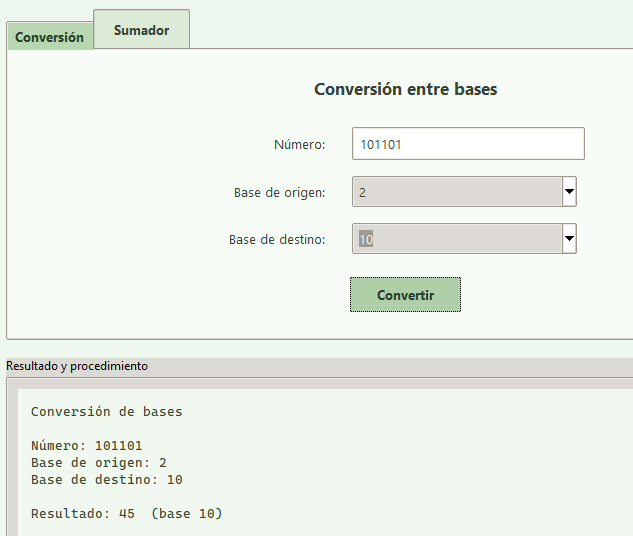
\includegraphics[width=0.75\textwidth]{img/ejecucion/01_conversion_entero.png}
    \caption{Conversi\'{o}n v\'{a}lida de un n\'{u}mero entero: $101101_2 = 45_{10}$.}
    \label{fig:conv_entero}
\end{figure}

\begin{figure}[H]
    \centering
    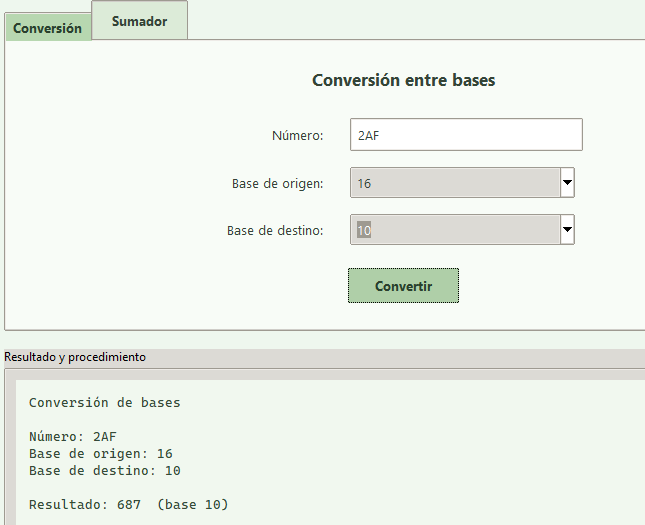
\includegraphics[width=0.75\textwidth]{img/ejecucion/02_conversion_fraccionaria.png}
    \caption{Conversi\'{o}n v\'{a}lida con parte fraccionaria: $10.625_{10} = 1010.101_2$.}
    \label{fig:conv_fraccionaria}
\end{figure}

\begin{figure}[H]
    \centering
    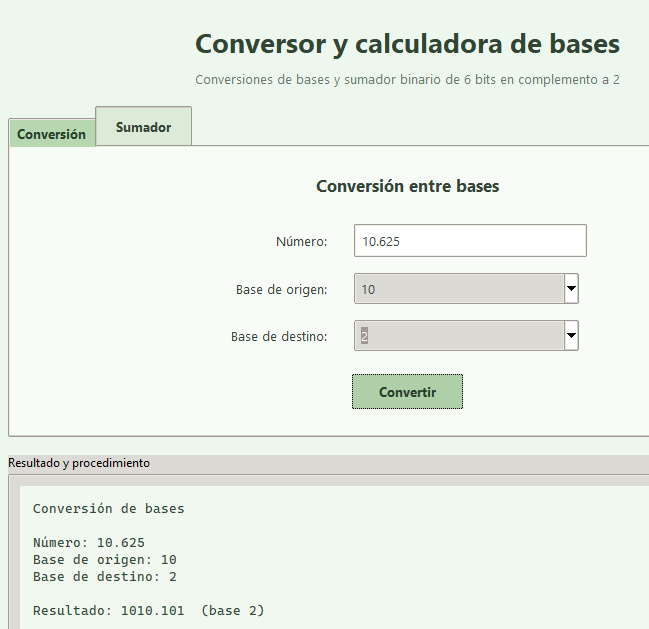
\includegraphics[width=0.75\textwidth]{img/ejecucion/03_conversion_letras.png}
    \caption{Conversi\'{o}n v\'{a}lida usando letras: $2AF_{16} = 687_{10}$.}
    \label{fig:conv_letras}
\end{figure}

\begin{figure}[H]
    \centering
    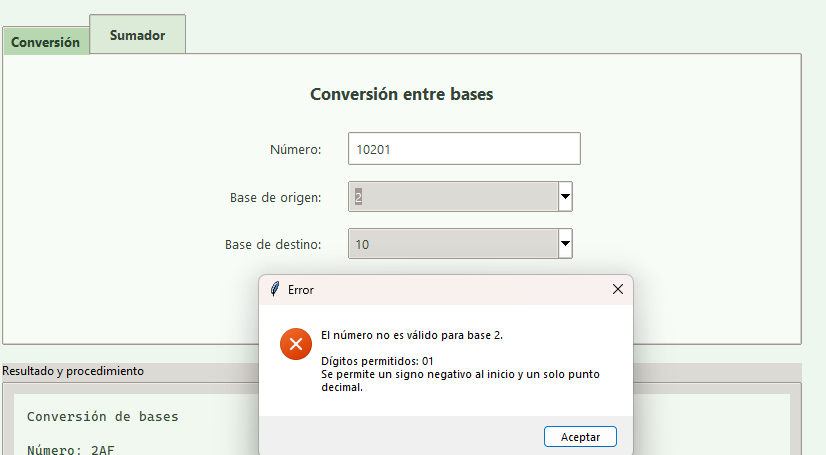
\includegraphics[width=0.75\textwidth]{img/ejecucion/04_validacion_digito_invalido.png}
    \caption{Validaci\'{o}n de un d\'{i}gito inv\'{a}lido: el n\'{u}mero $10201$ no es v\'{a}lido en base $2$.}
    \label{fig:validacion_digito}
\end{figure}

\begin{figure}[H]
    \centering
    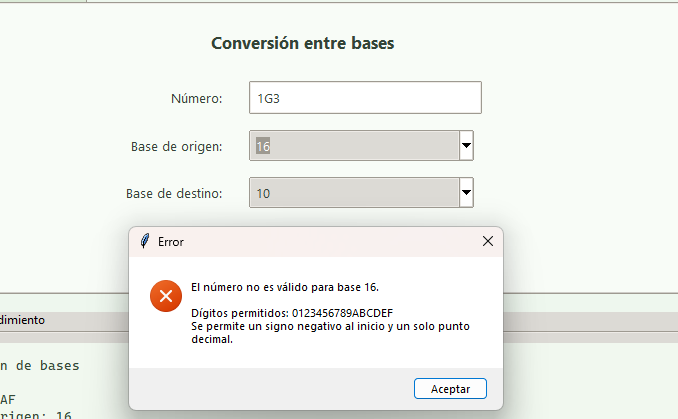
\includegraphics[width=0.75\textwidth]{img/ejecucion/05_validacion_letra_invalida.png}
    \caption{Validaci\'{o}n de una letra inv\'{a}lida: $G$ no es un d\'{i}gito v\'{a}lido en base $16$.}
    \label{fig:validacion_letra}
\end{figure}

\subsection{Casos del sumador}

La Figura~\ref{fig:suma_positivos} muestra la suma de dos positivos sin overflow; la Figura~\ref{fig:positivo_negativo} suma un positivo y un negativo; la Figura~\ref{fig:suma_negativos} suma dos negativos. Las Figuras~\ref{fig:overflow_positivos} y~\ref{fig:overflow_negativos} muestran el desbordamiento al sumar dos positivos y dos negativos, respectivamente; la Figura~\ref{fig:validacion_rango} el error al ingresar un valor fuera del intervalo y la Figura~\ref{fig:caso_limite} el caso l\'{i}mite $-32$.

\begin{figure}[H]
    \centering
    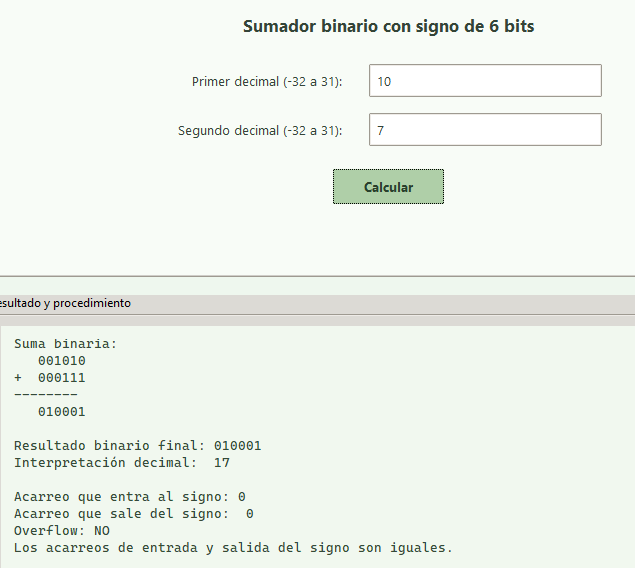
\includegraphics[width=0.75\textwidth]{img/ejecucion/06_suma_positivos_sin_overflow.png}
    \caption{Suma de dos positivos sin overflow: $10 + 7 = 17$.}
    \label{fig:suma_positivos}
\end{figure}

\begin{figure}[H]
    \centering
    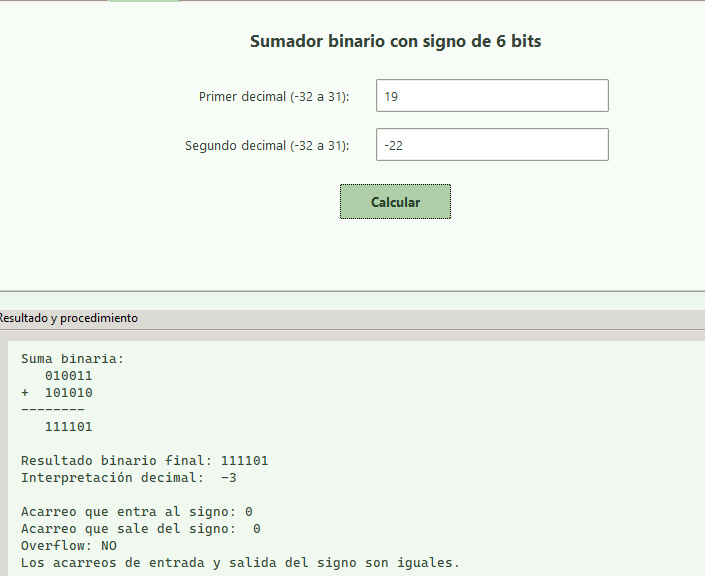
\includegraphics[width=0.75\textwidth]{img/ejecucion/07_positivo_negativo.png}
    \caption{Suma de un positivo y un negativo: $19 + (-22) = -3$.}
    \label{fig:positivo_negativo}
\end{figure}

\begin{figure}[H]
    \centering
    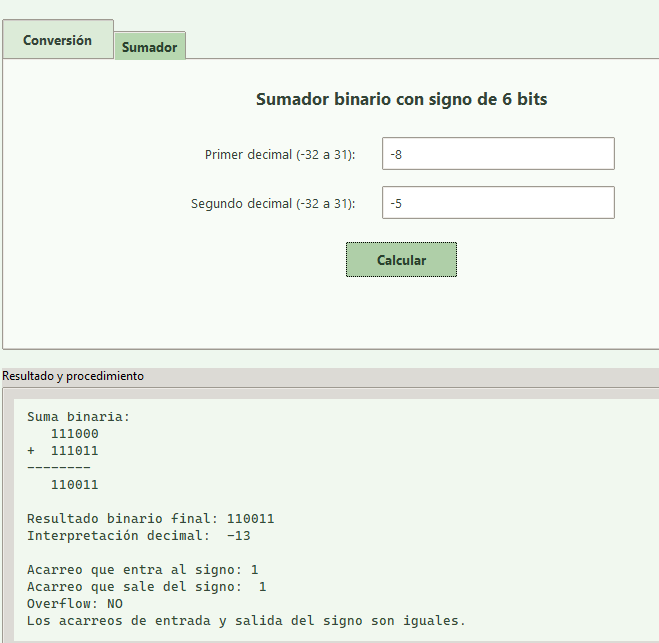
\includegraphics[width=0.75\textwidth]{img/ejecucion/08_suma_negativos.png}
    \caption{Suma de dos negativos: $-8 + (-5) = -13$.}
    \label{fig:suma_negativos}
\end{figure}

\begin{figure}[H]
    \centering
    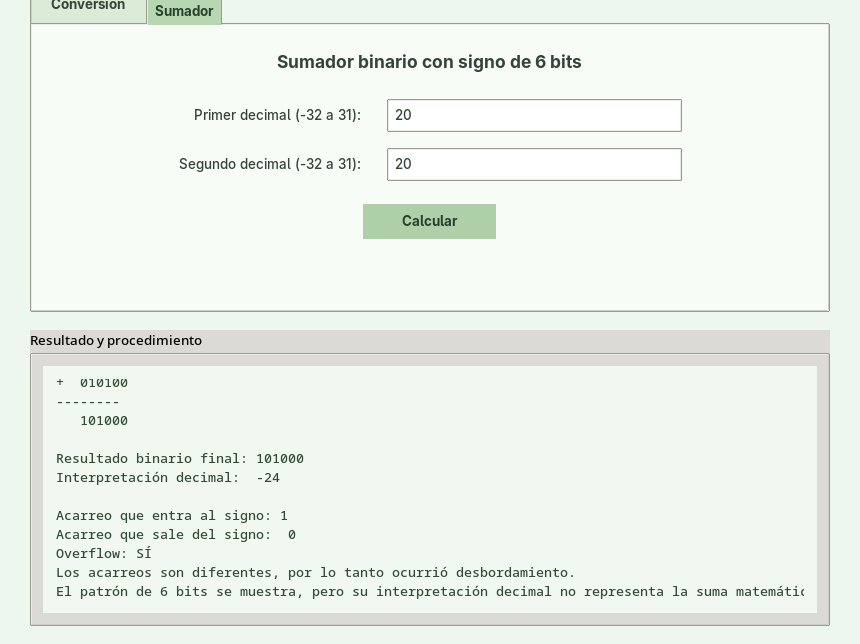
\includegraphics[width=0.75\textwidth]{img/ejecucion/09_overflow_positivos.png}
    \caption{Overflow al sumar dos positivos: $20 + 20 = 40$ excede el rango de $-32$ a $31$.}
    \label{fig:overflow_positivos}
\end{figure}

\begin{figure}[H]
    \centering
    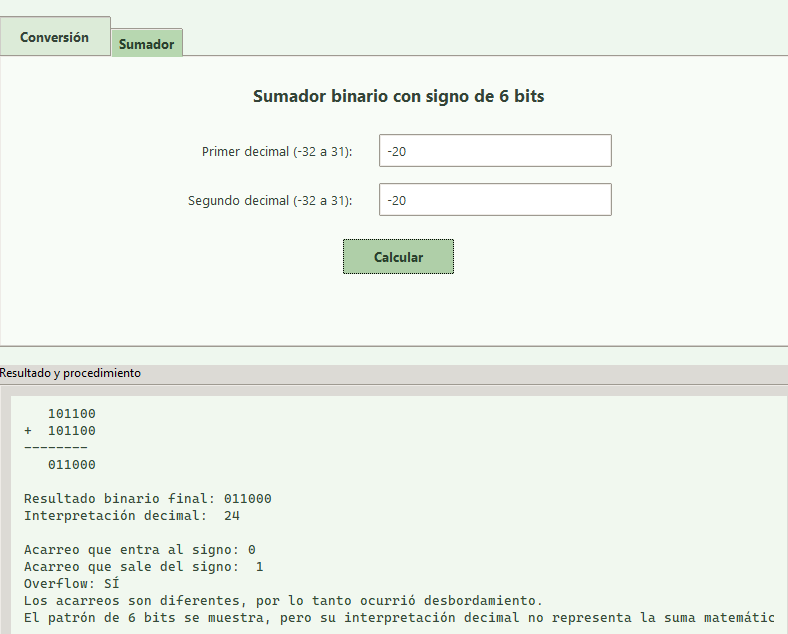
\includegraphics[width=0.75\textwidth]{img/ejecucion/10_overflow_negativos.png}
    \caption{Overflow al sumar dos negativos: $-20 + (-20)$ excede el rango de $-32$ a $31$.}
    \label{fig:overflow_negativos}
\end{figure}

\begin{figure}[H]
    \centering
    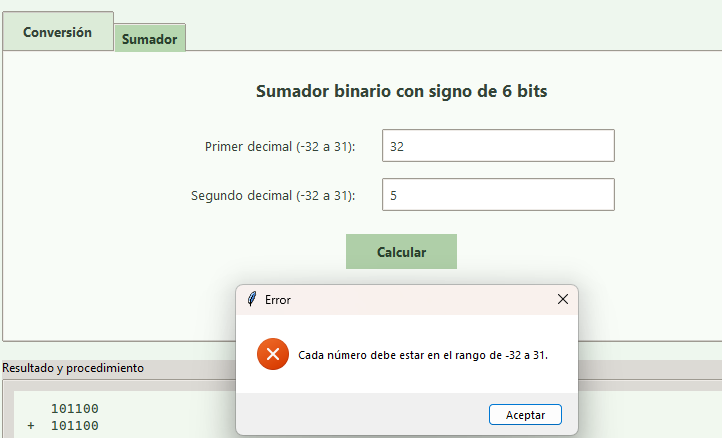
\includegraphics[width=0.75\textwidth]{img/ejecucion/11_validacion_rango_invalido.png}
    \caption{Validaci\'{o}n de rango: $32$ est\'{a} fuera del intervalo de $-32$ a $31$.}
    \label{fig:validacion_rango}
\end{figure}

\begin{figure}[H]
    \centering
    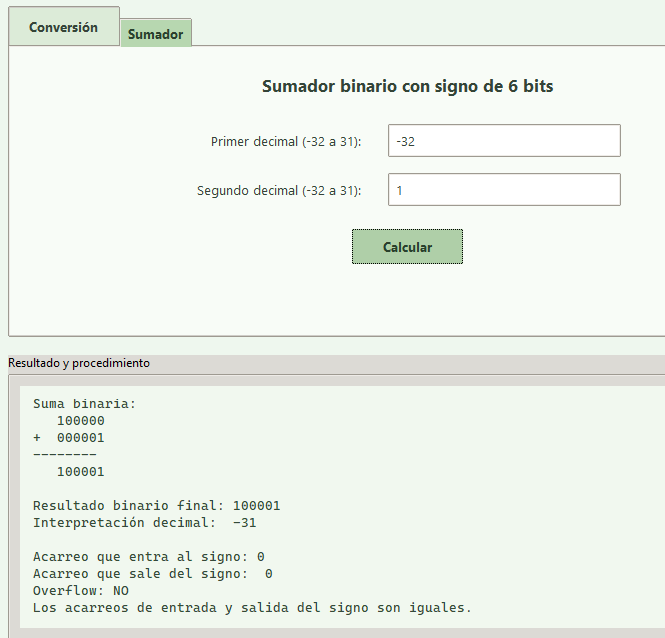
\includegraphics[width=0.75\textwidth]{img/ejecucion/12_caso_limite_menos32.png}
    \caption{Caso l\'{i}mite $-32$: se muestra su representaci\'{o}n especial $100000_2$; $-32 + 1 = -31$ sin overflow.}
    \label{fig:caso_limite}
\end{figure}

\end{document}
